\chapter{Wave Estimating Algorithm for Vessels Experiment (WEAVE)} \labchap{weave}

\section{Introduction} \labsec{weave_intro}

As a buoy is floats on top of waves, it experiences an acceleration proportional to the hydrodynamic forces exerted on it by $\pmb{F} = m\pmb{a}$. 
As a result, the buoy is displaced by a measurable amount as a wave passes through it. 
A wave buoy uses an accelerometer to measure the vertical acceleration component of this motion. 
By double integrating the signal with respect to time via the following equation, we can get the vertical displacement $z(t)$.

\begin{equation}
    z(t) = \frac{1}{2} a_z(t) \Delta t^2 + e
\end{equation}

Where $a_z(t)$ is the vertical acceleration time series, $\Delta t$ is the time since the last value update, and $e$ is the measurement error introduced by the sensor errors and integration errors (more on this later).

The equation shows that the error is multiplied over time, causing the reading to drift. 
Industry standard buoys like the DataWell WaveRider 4\footnote{https://datawell.nl/products/directional-waverider-4/} use high precision, regularly-calibrated sensors to minimize and account for the measurement error.

These types of uni-axial measurement buoys also rely on the measurement axis always being parallel to the Earth vertical axis. 
While the WaveRider 4 buoy accomplishes this by suspending the accelerometer on a platform in a fluid specifically tuned to act as a massive dampener, this comes at an increase to size and cost. 
Additionally, should this platform become misaligned to the global vertical axis, the measurements will always be of a component of the vertical acceleration and therefore introduce a bias in the calculations.

In this document, a procedure to use body frame coordinate rotation will be introduced that will eliminate the error and bias of a misaligned vertical axis measurement. 
The procedure will be implemented in two different ways: 1) a spectral analysis using the procedure laid out in Longuet-Higgins \cite{Longuet-Higgins:1963} and used by the WaveRider 4 buoy, 2) a novel oscillatory motion analysis based upon the work of Madgwick \cite{Gait-Tracking} that provides an instantaneous estimate of the wave height and direction.

\section{Background}
Inertial Measurement Units (IMUs) consist of an array of sensors that measure inertial forces acting on a body. 
Each measurement axis of the IMU is referred to as a degree of freedom (DOF). 
Advanced IMUs utilize 9 DOFs of measurements and also called Magnetic, Angular Rate, and Gravity (MARG) arrays. 
These sensors use a tri-axial magnetometer, gyroscope, and accelerometer, respectively to determine a body’s pose or orientation in 3D space, relative to a magnetic and gravitational field.

Using sensor fusion algorithms, it is possible to fuse the MARG array data into a unified representation of the body pose called the Attitude and Heading Reference System (AHRS). 
There are several such algorithms, most notably the complementary filter, the Kalman Filter, the Mahony filter, and the Madgwick filter. 
Madgwick’s filter is ideal for embedded applications because of its high accuracy, low performance cost, and ability to incorporate gyroscopic and magnetic drift compensation during runtime. 
This makes the attitude estimate over accurate over time and across a larger range of body motions. 
Therefore, this algorithm will be used exclusively during this study for sensor fusion.

\subsection{Quaternion Representation}

The crux of Madgwick’s filter is a gradient descent estimation of the body quaternion. 
The quaternion is a 4-dimensional representation of orientation that is free from infinite discontinuities found in 3-dimensional counterpart, Euler angles. 
The quaternion represents a 3D coordinate frame’s rotation about a unit vector in the base coordinate frame. 
his is represented graphically in the Figure \ref{fig:weave_frame_rotation} where the mutually orthogonal axes, $A_x$, $A_y$, $A_z$, $B_x$, $B_y$, $B_z$ represent the 3D frames $A$ and $B$, respectively.
When frame $B$ is rotated by some angle, $\theta$, about the unit vector, ${}^A \pmb{r}$, it now has an orientation relative to frame $A$ that can be expressed as the quaternion:

\begin{equation}
    {}^A_B\textbf{q} = \begin{bmatrix} q_1 & q_2 & q_3 & q_4 \end{bmatrix} = \begin{bmatrix} \cos\frac{\theta}{2} & -r_x\sin\frac{\theta}{2} & -r_y\sin\frac{\theta}{2} & -r_z\sin\frac{\theta}{2} \end{bmatrix}
\end{equation}

\begin{figure}[h!]
    \caption[Illustration of rotation between coordinates frame about an axis]{Illustration of the rotation from a base coordinate frame to a local coordinate frame about the axis, $\pmb{r}$}
    \labfig{weave_frame_rotation}
    \centering
    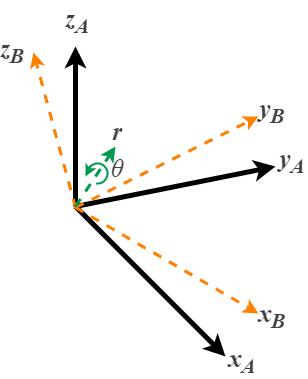
\includegraphics[height=1.5in]{background/frame_rotation.png}
\end{figure}

Note that we adopt the notation introduced by Craig \cite{Craig:2022}. 
The preceding superscript denotes the ``base'' or ``from'' coordinate frame and the preceding subscript denotes the ``derived'' or ``to'' coordinate frame. 
In the previous example, ${}_B^Aq$ is the quaternion representing the rotation \textit{from} frame $A$ \textit{to} frame $B$.

\subsection{Quaternion Application to Rotations}

If, by convention, we assume all bodies that are not Earth have some rotation relative to Earth’s central coordinate frame, then we can represent any body’s orientation as ${}^B_G\pmb{q}$ where $G$ is the global frame and $B$ is the body frame. 
If we also assume that the body is within Earth’s gravitational and magnetic field, then we can use a MARG array to determine ${}^B_G\pmb{q}$ via Madgwick’s filter.

Since quaternions represent coordinate frame rotations, we can use them to rotate 3D vectors from one frame to another. 
For example, in any given orientation in Earth’s gravitational field, there will always be components of gravitational acceleration within a body frame’s acceleration. 
Therefore, an accelerometer in the body frame will always be measuring the gravitational acceleration vector, ${}^G\pmb{a}$, and the body acceleration vector, ${}^B\pmb{a}$. 
If we want to eliminate the gravitational signal, we can rotation the gravitational acceleration vector from the global coordinate frame to the body frame and subtract it from our readings. 
This will yield the body linear accelerations, ${}^B\pmb{a}_l$, defined as:

\begin{gather}
    {}^G_B\pmb{a} = {}^G_B\pmb{q} \cdot {}^G\pmb{a} \cdot {}^G_B\pmb{q}^{-1} \\
    {}^B\pmb{a}_l = {}^B\pmb{a} - {}^G_B\pmb{a}
\end{gather}

Again, using the notation from Craig to denote the ``from'' and ``to'' frames, respectively. Also note that ${}^G_B\pmb{q}^{-1}$ is the inverse quaternion as defined by:

\begin{equation*}
    {}^G_B\pmb{q}^{-1} = \begin{bmatrix} -q_1 & -q_2 & -q_3 & -q_4 \end{bmatrix}
\end{equation*}

Alternatively, we can rotate the body accelerations to the global frame and get global linear accelerations, ${}^B_G\pmb{a}_l$, via a similar operation:

\begin{gather}
    {}^B_G\pmb{a} = {}^B_G\pmb{q} \cdot {}^B\pmb{a} \cdot {}^B_G\pmb{q}^{-1} \\
    {}^B_G\pmb{a}_l = {}^B_G\pmb{a} - {}^G\pmb{a}
\end{gather}

By convention, the global coordinate frame is typically referred to as North-East-Down (NED) and therefore, ${}^G\pmb{a} = \begin{bmatrix} 0 & 0 & 1 \end{bmatrix}$

\section{Spectral Analysis Theory}

For the spectral analysis, the work by Longuet-Higgins will be heavily utilized. 
The displacement vector should be subsampled to 2.56 Hz. 
Over a 200-second interval, a total of $N=512$ samples are collected. 
We can then obtain a frequency spectrum via the Fast Fourier Transform (FFT). 
The spectrum will have a range of $0$ to $\frac{f_s}{2}=1.28 \text{Hz}$ and a resolution of $\frac{f_s}{N}=0.005 \text{Hz}$.
The FFT yields Fourier coefficients via:

\begin{equation}
    \sum_{k=0}^{N-1} w_k h_k e^{\frac{2\pi kl}{N}}
\end{equation}

Where $f_l=\frac{1}{N\Delta t}$ and $= 0 \ldots N-1$ and the $w_k$ element is a windowing function. 
Datawell uses a Hann windowing function \cite{WaveRider4UserManaul} which attenuates signals in the higher frequency domains:

\begin{equation}
    w_k = \frac{1}{2} [1-\cos{\frac{2\pi k}{N}}] \text{ where } k=0 \ldots N-1
\end{equation}

We can normalize these coefficients via:

\begin{equation}
    w_{norm} = \sqrt{f_s \sum_{k=0}^{N-1}w_k^2}
\end{equation}

Since we have time series data for all three axes, we can take the spectra for each series. 
Each series contains a vector of coefficients and can be expressed in vector notation as:

\begin{align}
    a_N &= \alpha_N + i\beta_N \\
    a_E &= \alpha_E + i\beta_E \\
    a_D &= \alpha_D + i\beta_D
\end{align}

We can then define the co-spectra ($C$) and the quad-spectra ($Q$) as follows:

\begin{gather}
    C_{xy} = a_x \cdot a_y = \alpha_x \alpha_y + \beta_x \beta_y \\
    C_{xy} = a_x \times a_y = \alpha_x \beta_y - \beta_x \alpha_y
\end{gather}

Then, we can arrange them into 3 by 3 matrices to obtain the final definition of the acceleration spectra:

\begin{gather}
    \begin{bmatrix}
        C_{NN} & C_{NE} & C_{ND} \\
        C_{EN} & C_{EE} & C_{ED} \\
        C_{DN} & C_{DE} & C_{DD}
    \end{bmatrix} \\
    \begin{bmatrix}
        0 & 0 & Q_{ED} \\
        0 & 0 & Q_{ND} \\
        Q_{DE} & Q_{DN} & 0
    \end{bmatrix}
\end{gather}

Note that by definition, $Q_{NN}=Q_{EE}=Q_{DD}=0$ and $Q_{EN}$ and $Q_{NE}$ represent eddy currents and are not considered.

These spectra can represent different wave parameters such as wave direction, direction spread, wave ellipticity, and power spectral density (PSD). 
The wave direction, $\theta_0$, is defined as the angle from which the waves are approaching relative to geographic north.

\begin{equation}
    \theta_0 = \arctan{\frac{-Q_{ED}}{Q_{ND}}}
\end{equation}

The direction spread can be more difficultly determined via:

\begin{gather}
    S = \sqrt{2-2m_1} \\
    \begin{aligned}
        \text{where }   &m_1 = \sqrt{a_1^2 + b_1^2} \\
                        &a_1 = \frac{Q_{ND}}{\sqrt{(C_{NN}+C_{EE})C_{DD}}} \\
                        &b_1 = \frac{-Q_{ED}}{\sqrt{(C_{NN}+C_{EE})C_{DD}}}
    \end{aligned}
\end{gather}

The wave ellipticity describes the shape of the wave. 
Specifically, the particle trajectories. 
For wavelengths much smaller than the water depth, the particles will follow a circular trajectory, thus the ellipticity is near 1. 
However, as the wavelength approaches the water depth, the vertical displacements reduce and the ellipticity becomes less than 1, trending towards 0. 
We can determine this parameter via:

\begin{equation}
    \epsilon = \frac{1}{k} = \sqrt{\frac{C_{DD}}{C_{NN}+C_{EE}}}
\end{equation}

Finally, the PSD describes the amount of energy present in the signal across the entire frequency spectrum. 
The PSD for the vertical axis is considered the wave spectrum and is calculated by:

\begin{equation}
    E(f) = C_{DD} = \alpha^2_D + \beta^2_D
\end{equation}

By taking the integral of the PSD we can find the n-th spectral moment of the signal. 
The zeroth spectral moment, $m_0$, can tell us a lot of information such as the significant wave height, $H_s$, and the peak wave period, $T_p$.

\begin{gather}
    m_0 = \int^\infty_0 f^0E(f)df \\
    H_s = 4\sqrt{m_0} = H_{m_0} \\
    T_p = 5 \sqrt{H_s}
\end{gather}

\section{Oscillitory Motion Tracking Theory}

The spectral analysis method is the industry standard and recommended by NOAA \cite{NOAAWaveMeasure}. 
However, the spectra needs to be analyzed over time. 
The accuracy of the spectral analysis directly correlates with its sample interval; instantaneous intervals will never be completely representative whereas infinite intervals will be 100\% accurate.
The above methodology offers a balance of accuracy and reporting time. 
But, the sample interval of 200-seconds may be too long for some applications. 
Therefore, in this section we will explore an alternative approach where the wave height is directly computed instantaneously using accelerometer integration and feedback error correction.

We start by using the rotated linear accelerations derived in the Section \ref{sec:weave_intro}. 
These can be integrated over time to get velocity, $\pmb{v}$, as shown below:

\begin{equation}
    {}^G\pmb{v}(t) = {}^G\pmb{a}(t) \Delta t
\end{equation}

The integration error accumulates over time and causes the signal to drift, or deviate from the true value. 
We can consider this drift a velocity signal with infinite period and apply a high-pass filter with an extremely small cutoff frequency to attenuate the error. 
The filter design is discussed in an upcoming subsection. 
We can perform another integration to get the buoy displacement in the global frame:

\begin{equation}
    {}^G\pmb{s}(t) = {}^G\pmb{v}(t)\Delta t + \pmb{e} = {}^G\pmb{a}(t) \Delta t^2 + \pmb{e}
\end{equation}

The integration error for displacement is also fed by the error from velocity, so this value will drift faster over time. 
Again, we can consider the drift an infinite period signal and apply another high-pass filter. 
Madgwick, 2013 shows this method is effective for motions where a zero-velocity point occurs (e.g. at the bottom of a step). 
But, this method needs to be tested on a constantly moving object, like a wave buoy.

\subsection{Filter Design}
The goals of the velocity and displacement filters are to maximize the attenuation of the error signal while minimizing both the attenuation of the desired signal and the induced phase shift. 
The ideal filter will have these criteria, but they are impossible to design. 
Therefore, we must compromise between the two.

There are four main digital infinite impulse response filters: Bessel, Butterworth, Chebyshev (Type I and Type II), and Elliptic. 
Each filter can be expressed by its ``order'' or how many times the filter is applied to the signal. 
The higher the order, the steeper the transition and the closer the magnitude response becomes to ideal. 
But, this often comes at the cost of dramatically increasing phase shift. 
The main filters can generally be ranked in the order given above: from left to right, the transition becomes steeper with a smaller order; from right to left, the phase shift is more linear in the pass band.

If a more linear/minimized phase shift is desired, then a low order Bessel or Butterworth filter is best. 
Though, their transition areas can span many frequency decades. 
Since our cutoff frequency is extremely small, we want the most reactive filter with the narrowest transition. 
To make the Bessel and Butterworth filter fulfill this criterion, we need to substantially increase their orders, eliminating their beneficial phase shift characteristic.

The two remaining filters, Chebyshev and Elliptic, have sharper transition regions but at the cost of non-linear phase shifts and ripple in the pass and stop bands. 
For a bandpass filter design, we can define a couple of parameters: a low-stop frequency of 0.025 Hz, a low-pass frequency of 0.05 Hz, a high-stop frequency of 2.0 Hz, a high-pass frequency of 0.25 Hz, a stop attenuation of 100 dB, and a pass attenuation of 0.1 dB. 
With these values, different bode plots for Chebyshev Type I (Figure \ref{subfig:chebyshev_1}), Chebyshev Type II (Figure \ref{subfig:chebyshev_2}), and Elliptic (Figure \ref{subfig:elliptic}) filters were created.

\begin{figure}[h!]
    \centering
    \subfloat[Chebyshev Type I filter]{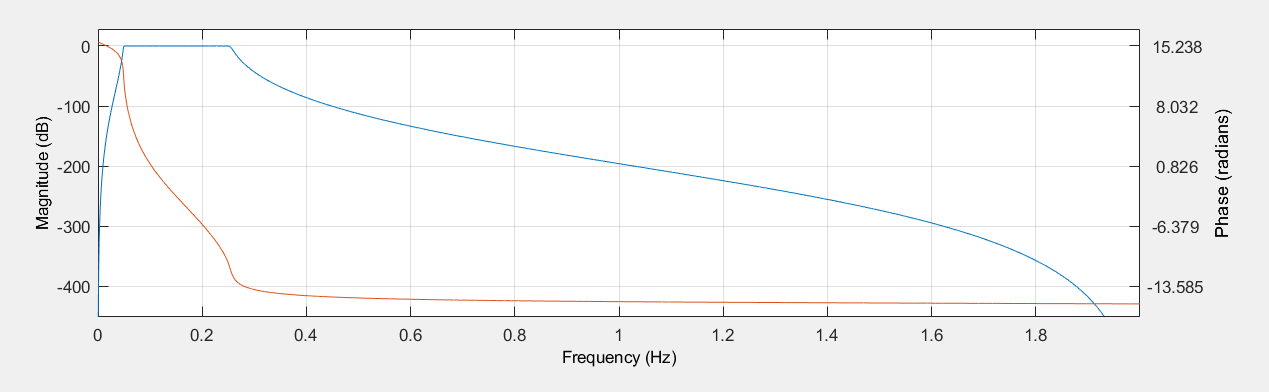
\includegraphics[height=1.5in]{appendices/weave/chebyshev_1.png}\label{subfig:chebyshev_1}}\hskip3ex
    \subfloat[Chebyshev Type II filter]{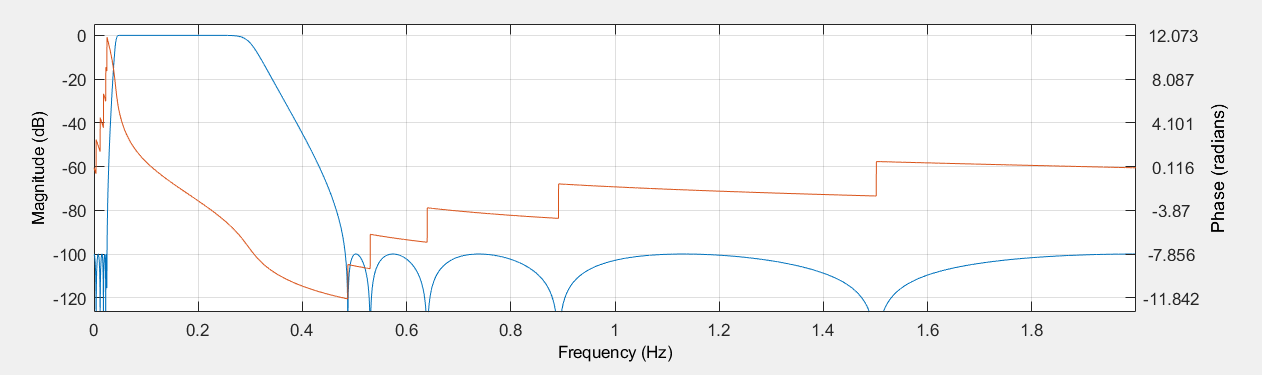
\includegraphics[height=1.5in]{appendices/weave/chebyshev_2.png}\label{subfig:chebyshev_2}}\hskip3ex
    \subfloat[Elliptic filter]{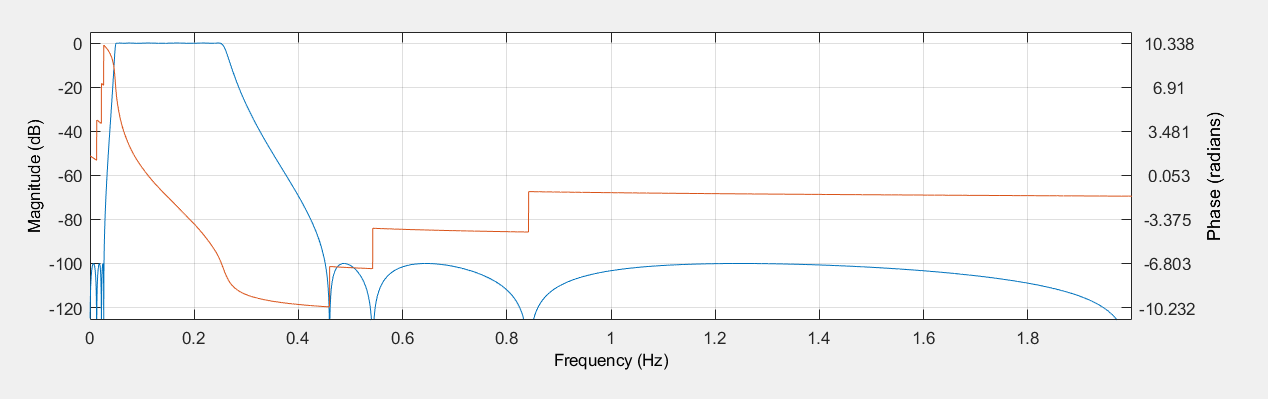
\includegraphics[height=1.5in]{appendices/weave/elliptic.png}\label{subfig:elliptic}}\hskip3ex
    \caption[Digital filter bode plots]{Bode plots for Chebyshev and Elliptical filters using a low-stop frequency of 0.025 Hz, a low-pass freuqnecy of 0.05 Hz, a high-stop frequency of 2.0 Hz, a high-pass frequency of 0.25 Hz, a stop attenuation of 100 dB, and a pass attenuation of 0.1 dB.}
    \labfig{filter_bode_plots}
\end{figure}

From these plots, we can see that the both the Chebyshev Type II and Elliptic filter have undesired ripple on the stop bands and the phase shift is very non-linear. 
The Chebyshev Type I filter on the other hand has a much sharper attenuation of the stop bands without any ripple at the cost of some more phase shift. 
We will therefore be using the Chebyshev Type I filter for our analysis.

\section{Methodology}
The two wave analysis techniques will be performed in post-processing after a data collection period. 
Data will be collected using the Thetis inertial datalogger and the x-IMU3 datalogger \cite{xioTechnologies}. 
The devices will be rigidly attached to the top of a Datawell WaveRider4 buoy and will be accepted as the ground truth for the experiment and used to validate the spectral analysis procedure.

The devices will be deployed for a total of six hours on five different days since the batteries have to be recharged after that length of deployment. 
Data will be offloaded and stored onto a computer after recovery. 
Both Thetis and the x-IMU3 will supply data at 64 Hz meaning each batch of data contains 1.4 million points for a total of 6.9 million data points. 
Using the Madgwick filter, the data points will be used to compute the buoy orientation and linear acceleration over time.

\subsection{For Spectral Analysis}
The linear acceleration dataset wil be subsampled from 64 Hz to about 2.56 Hz using a rolling average filer of $N=25$ samples. 
This will eliminate most of the high frequency noise while still preserving the wave motion signal. 
From here, the data analysis procedure from the previous section will be used to calculated the wave statistics, averaged over each hour of runtime. 
These can be directly compared to the data pulled from the wave buoy using a Root Mean Square Error ($RMSE$) as shown below:

\begin{equation}
    RMSE_H = \sqrt{\frac{\sum{(H_{sX}-H_{sB})^2}}{N}}
\end{equation}

Where $H_{sX}$ is the significant wave height calculated by the inertial data loggers, $H_{sB}$ is the significant wave height reported by the buoy, and $N$ is the number of samples.

\begin{equation}
    RMSE_T = \sqrt{\frac{\sum{(T_{pX}-T_{pB})^2}}{N}}
\end{equation}

Where $T_{pX}$ is the significant wave height calculated by the inertial data loggers, $T_{pB}$ is the significant wave height reported by the buoy, and $N$ is the number of samples.

Note that due to the limited sample time, the comparisons are only valid for a small wave regime. 
The results section will detail the validity more in-depth, but for a more accurate analysis, these instruments must be deployed for longer under a wider array of waves.

\subsection{For the Oscillatory Motion Tracking Analysis}

The data will again be subsampled to about 4 Hz using a rolling average filer of $N=16$. 
As before, this eliminates high frequency noise while preserving the much lower frequency wave motion signals (this can help prevent drift throughout the analysis).

We can take the first integral of our linear acceleration data which yields the buoy’s linear velocities plus errors in the global frame. 
These can be filtered out by applying a bandpass Chebyshev Type I filter to the data. 
By observation of the Rayleigh Distribution for waves, we can assess that a majority of wave-related motion will occur in the 4- to 20-second range. 
We can therefore tailor the filter such that we have the sharpest cut-off around the range of our expected signal frequency while maximizing the stopband attenuation.

After applying the filter to the velocity data, we cna take the integral again to yield the buoy displacement in the global frame. 
The same bandpass filter as used before can be applied to this new time series which will give us the best estimate of the buoy’s displacement. 
The vertical displacement series represents the sea surface elevation time series, $\eta$.

From the displacement, we can perform a wave-by-wave analysis which uses the zero-upcrossing method to identify discrete windows of a wave. 
The psuedocode for the algorithm is given below. 
The analysis of all these windows yields wave statistics that we can compare between the inertial data loggers and the spectral analysis method.

\begin{algorithm}
    \begin{algorithmic}[1]
        \Function{WaveByWave}{$\eta,f_s,g$}
        \State index $\longleftarrow 1$
        \State negIndices $\longleftarrow$ find all negative indices in $\eta$ \Comment{negIndices is a list of indicies}
        \For{n=1, $\dots$, size(negIndices)}
            \If{$\eta$[negIndices[n]+1]$ > 0$}
                \State upcrossTimes[index] $\longleftarrow$ negIndices[n]
                \State index++
            \EndIf
        \EndFor

        \For{u=1, $\dots$, size(upcrossTimes)-1}
            \State $\eta_u \longleftarrow \eta$[upcrossTimes[u]:upcrossTimes[u+1]]
            \State Calculate $H_u$, $T_u$, and others for $\eta_u$
            \State Put wave parameters into wave structure
            \State Append the new wave structure to $waves$
        \EndFor
        \State Return $waves$
        \EndFunction
    \end{algorithmic}
    \caption{Wave By Wave}\label{alg:wave_by_wave}
\end{algorithm}

This method is not flawless as statistically insignificant up-crossings called, false peaks, will be detected and recorded. 
We can filter out the false peaks by following the methodology laid out in Coats \cite{Coats:2013}. 
We can compute the root mean square of the wave heights using the equation below. 
Then, we can filter out all of the waves which height fall below the arbitrary threshold $0.1H_{\text{rms}}$.

\begin{equation}
    H_{\text{rms}} = \sqrt{\frac{1}{N} \sum{H_i^2}}
\end{equation}

Additionally, we can remove false peaks by examining the time between them. 
From Rayleigh \cite{DeanAndDalrymple}, we can be confident that the wave period will not be faster than 4-seconds, nor slower than 20-seconds. 
Therefore, any peaks that occur within 4-seconds of or 20-seconds after another can be discarded. 
After we remove all the false peaks, the array of waves must be sorted in descending order according to their height.

From the wave-by-wave analysis, we can determine the significant wave height by calculating the highest one third of wave heights using:

\begin{equation}
    H_s = H_{\frac{1}{3}} = \frac{3}{N} \sum_{i=\frac{2}{3}N}^N H_i
\end{equation}

If we want to directly compare to the previous methods, we need to window our waves in the same time periods as the spectral analysis. 
We can compute the significant wave height for that window using the above equation and determine the peak period by creating a distribution of periods (that is, time between upcrossings) in that window; the peak wave period would be that with the most counts in its bin. 
As before, we can compare the inertial data loggers to each other via per cent difference, and to the wave buoy via the RMSE method.